% technical background

% sample latex/latex2e file with lots of math, tables, figures, etc
% useful for writing papers
% genuine finger-typed files by Christina C. Christara

\documentclass[12pt]{article}
% \documentclass[12pt]{mypaper}

%\linespread{1.1} % for more than single spacing

% take more advantage of the size of paper
\addtolength{\topmargin}{-2cm}
\addtolength{\textheight}{4cm}
\addtolength{\evensidemargin}{-2cm}
\addtolength{\oddsidemargin}{-2cm}
\addtolength{\textwidth}{4cm}

% some standard packages
\usepackage{times}
\usepackage{graphics}
\usepackage{subfigure, epsfig}
\usepackage{rotate}
\usepackage{amssymb}
\usepackage{amsmath}
\usepackage{natbib} % bib
\usepackage{tikz} % neural networks
\usetikzlibrary{matrix,chains,positioning,decorations.pathreplacing,arrows}


\setlength{\parskip}{3mm}
% convenient abbreviations
\newcommand{\de}{\partial}
\newcommand{\mb}{\mathbf}

\begin{document}


\Large
{\bf Background}

\normalsize
This document will explore the technical details of a feed-forward 
neural network, and an application for recognizing hand-written digits.

In the simplest case, neural networks can be reduced to 
a generalized linear model (GLM),
where the prediction is a linear combination of inputs
but passed through a non-linear function:
%
\begin{equation}
	f(\mb{x},\mb{w}) = g\left( \sum_{i=1}^N w_i x_i \right)
\end{equation}
%
\indent Here $g(\cdot)$ is a non-linear function, 
with $\mb{x}$ is an $N$ dimensional input vector,
and $\mb{w}$ is the weight vector.
Common choices of $g(\cdot)$ for neural networks 
include the logistic (sigmoid) function, the hyperbolic tangent function, 
and the rectified linear unit (ReLU):
%
\begin{equation}
\begin{aligned}
	g_{\text{logistic}}(z) &= \frac{1}{1+e^{-z}} \\
	g_{\text{tanh}}(z) &= \tanh(z) = \frac{1 - e^{-2x}}{1 + e^{-2x}}\\
	g_\text{ReLU}(z) &= \max(z,0)
\end{aligned}
\end{equation}
%
\indent 
Notice all of these functions have simple derivatives,
and specifically logistic and hyperbolic tangent functions 
map to bounded ranges,
which are great choices for classification problems.

Graphically, this can be represented by a series of 
input nodes $\{x_i\}$ connected to an output node $f$,
with weights $\{w_i\}$ on the connections.

\def\layersep{2.5cm}
\begin{figure}[h]
\centering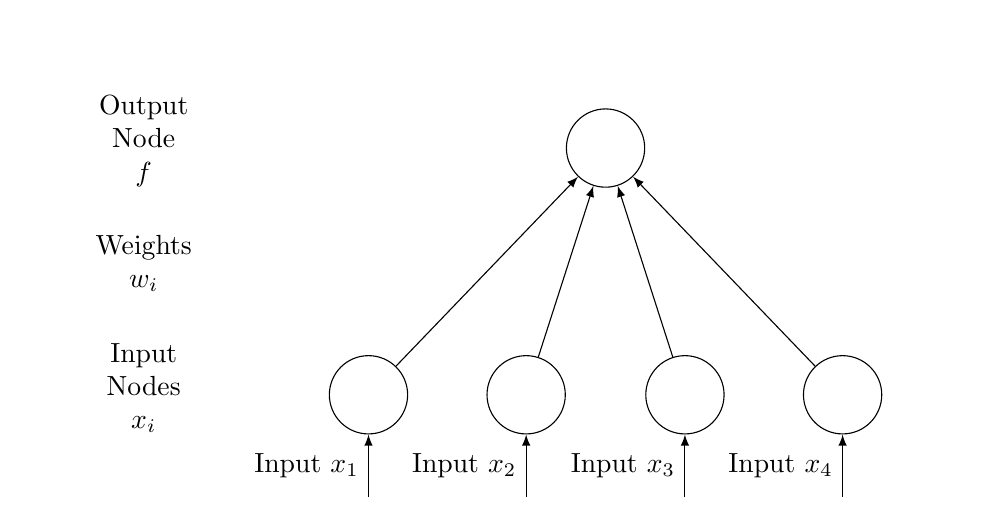
\begin{tikzpicture}[
plain/.style={
  draw=none,
  fill=none,
  },
net/.style={
  matrix of nodes,
  nodes={
    draw,
    circle,
    inner sep=10pt
    },
  nodes in empty cells,
  column sep=0pt,
  row sep=-1cm
  },
>=latex
]

\matrix[net] (mat)
{
|[plain]| \parbox{1.2cm}{\centering Output Node\\$f$} & |[plain]| & 
    |[plain]| & |[plain]| & |[plain]| & & |[plain]| & |[plain]| & |[plain]| 
    & |[plain]| \\
|[plain]| \parbox{1.3cm}{\centering Weights\\$w_{i}$}
    &|[plain]| &|[plain]| &|[plain]| &|[plain]| &
    |[plain]| &|[plain]| &|[plain]| &|[plain]| &|[plain]| \\
|[plain]| \parbox{1.3cm}{\centering Input Nodes\\$x_i$} & 
    |[plain]| & & |[plain]| & & |[plain]| & & |[plain]| &\\
};
\foreach \ai [count=\mi ]in {3,5,7,9}
  \draw[<-] (mat-3-\ai) -- node[left] {Input $x_\text{\mi}$} +(0cm,-1.3);
\foreach \ai in {6}
{\foreach \aii in {3,5,7,9}
  \draw[<-] (mat-1-\ai) -- (mat-3-\aii);
}
\end{tikzpicture}

\caption{\label{fig:GLM}
A generalized linear model represented in graphical form.
In a neural network, this is also referred to as a single neuron.
}
\end{figure}

%formatting
\pagebreak

A general feed-forward neural network is defined by recursive GLMs
with different weights.
For example, a neural network with two hidden layers
(three layers of recursion) is defined as:
%
\begin{equation}
\begin{aligned}
	h^{(1)}_j &= g^{(1)}
		\left(\sum_{i=1}^{N^{(1)}} w_{ij}^{(1)} x_i \right) \\
	h^{(2)}_k &= g^{(2)}
		\left(\sum_{j=1}^{N^{(2)}} w_{jk}^{(2)} h_j^{(1)} \right) \\
	f_l &= g^{(3)}
		\left(\sum_{k=1}^{N^{(3)}} w_{kl}^{(3)} h_k^{(2)} \right)
\end{aligned}
\end{equation}
%
where $g(\cdot)^{(\alpha)}$ is some activation function,
$h^{(\alpha)}_j$ denotes the $j^\text{th}$ node of the $\alpha^\text{th}$ 
hidden layer,
$w_{ij}^{(\alpha)}$ denotes the weight for the connection of 
the $i^\text{th}$ node of the $\alpha^\text{th}$ layer to 
the $j^\text{th}$ node of the $(\alpha+1)^\text{th}$ layer,
and $N^{(\alpha)}$ denotes the number of nodes in the $\alpha^\text{th}$ layer.

Graphically, this structure has a very clear representation:
%
\def\layersep{2.5cm}
\begin{figure}[h]
\centering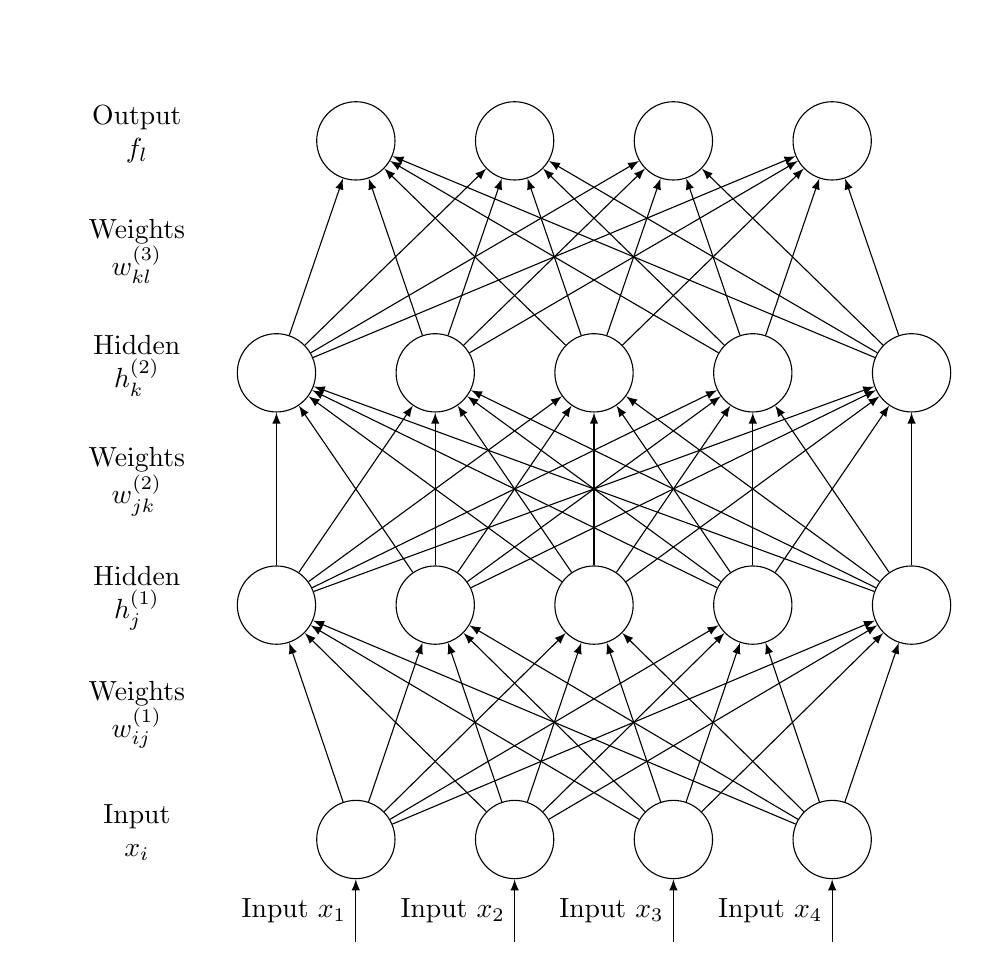
\begin{tikzpicture}[
plain/.style={
  draw=none,
  fill=none,
  },
net/.style={
  matrix of nodes,
  nodes={
    draw,
    circle,
    inner sep=10pt
    },
  nodes in empty cells,
  column sep=0pt,
  row sep=-1cm
  },
>=latex
]

\matrix[net] (mat)
{
|[plain]| \parbox{1.3cm}{\centering Output\\$f_l$} & 
    |[plain]| & & |[plain]| & & |[plain]| & & |[plain]| &\\
|[plain]| \parbox{1.3cm}{\centering Weights \\$w_{kl}^{(3)}$}\\
    % &|[plain]| &|[plain]| &|[plain]| &|[plain]| &
    % |[plain]| &|[plain]| &|[plain]| &|[plain]| &|[plain]| \\
|[plain]| \parbox{1.2cm}{\centering Hidden\\$h_k^{(2)}$} & & 
    |[plain]| & & |[plain]| & & |[plain]| & & |[plain]| & \\
|[plain]| \parbox{1.3cm}{\centering Weights \\$w_{jk}^{(2)}$}
    &|[plain]| &|[plain]| &|[plain]| &|[plain]| &
    |[plain]| &|[plain]| &|[plain]| &|[plain]| &|[plain]| \\
|[plain]| \parbox{1.2cm}{\centering Hidden\\$h_j^{(1)}$} & & 
    |[plain]| & & |[plain]| & & |[plain]| & & |[plain]| & \\
|[plain]| \parbox{1.3cm}{\centering Weights \\$w_{ij}^{(1)}$}
    &|[plain]| &|[plain]| &|[plain]| &|[plain]| &
    |[plain]| &|[plain]| &|[plain]| &|[plain]| &|[plain]| \\
|[plain]| \parbox{1.3cm}{\centering Input\\$x_i$} & 
    |[plain]| & & |[plain]| & & |[plain]| & & |[plain]| &\\
};
\foreach \ai [count=\mi ]in {3,5,7,9}
  \draw[<-] (mat-7-\ai) -- node[left] {Input $x_\text{\mi}$} +(0cm,-1.3);
\foreach \ai in {3,5,7,9}
{\foreach \aii in {2,4,...,10}
  \draw[<-] (mat-1-\ai) -- (mat-3-\aii);
}
\foreach \ai in {2,4,...,10}
{\foreach \aii in {2,4,...,10}
  \draw[<-] (mat-3-\ai) -- (mat-5-\aii);
}
\foreach \ai in {2,4,...,10}
{\foreach \aii in {3,5,7,9}
  \draw[<-] (mat-5-\ai) -- (mat-7-\aii);
}
\end{tikzpicture}

\caption{\label{fig:NN}
A generalized feed-forward neural network with two hidden layers.
}
\end{figure}

% formatting
\pagebreak 

While most GLMs do not admit a closed-form solution,
a satisfactory optimization can be achieved by the gradient descent method.
In the neural network case,
the optimization becomes more difficult as
the number of parameters increase with the number of nodes and layers.
However, we can still apply the gradient descent method
and find a local optimum.

Suppose we have a dataset $\mathcal{D} = \{\mb{x}^{[n]}, 
\mb{y}^{[n]}\}, n \in \mathbb{N}$,
and we want to find a model $f(\mb{x},\mb{w})$ such that 
it is the ``closest'' to $\mb{y}$.
Given a differentiable error function $E(f,\mb{y})$
and model $f(\mb{x},\mb{w})$ with respect to $\mb{w}$,
the model can be optimized by gradient descent.
In other words, for any randomly initialized $\mb{w}^0$,
an improvement can be obtained by taking a step towards 
the direction of the gradient with respect to $\mb{w}^k$ :
%
\begin{equation}
	\mb{w}^{k+1} = \mb{w}^{k} - \eta \; \nabla_{\mb{w}^k} 
					E\left(f(\mb{x},\mb{w}^k),\mb{y}\right)
\end{equation}
%
where $\eta$ is a constant controlling the size of 
each optimization step, commonly called the learning rate.

In the the two hidden layer neural network previously,
a derivative with respect to any $w_{ij}^{(\alpha)}$ can be found
through chain rule of the derivatives.
For example the derivative with respect to $w_{jk}^{(2)}$ :
%
\begin{equation}
\begin{aligned}
	\text{let } z_j^{(\alpha)} &= 
		\sum_{i=1}^{N^{(\alpha)}} w_{ij}^{(\alpha)} h_i^{(\alpha-1)} \\
	\text{then } \frac{\de E}{\de w_{jk}^{(2)}} &= 
		\sum_{l=1}^{N^{(4)}} \frac{\de E}{\de f_l}
		\frac{\de f_l}{\de z_l^{(3)}}
		\frac{\de z_l^{(3)}}{\de h_k^{(2)}}
		\frac{\de h_k^{(2)}}{\de z_k^{(2)}}
		\frac{\de z_k^{(2)}}{\de w_{jk}^{(2)}} \\
	&=
		\sum_{l=1}^{N^{(4)}} \frac{\de E}{\de f_l}
		\frac{\de g^{(3)}(z_l^{(3)}) } {\de z_l^{(3)}}
		w_{kl}^{(3)}
		\frac{\de g^{(2)}(z_k^{(2)}) } {\de z_k^{(2)}}
		h_j^{(1)} .
\end{aligned}
\end{equation}
%
% \indent 
Recall $g^{(\alpha)}(\cdot)$ is selected to have a simple derivative,
making the complex appearing expression above easy to compute.

A common technique to improve speed of convergence is by adding momentum.
The idea is to let the gradient dictate the acceleration of 
the change in $\mb{w}^k$ instead of the velocity.
This allows the optimization to move faster in the direction
of the gradient, while making it harder to converge to a poor local minimum.
The formulation starts with a velocity vector $\mb{v}^0$
initialized to zero, and the rest in similar:
%
\begin{equation}
\begin{aligned}
	\mb{v}^{k+1} &= \mb{v}^{k} - \eta \; \nabla_{\mb{w}^k} 
				E\left(f(\mb{x},\mb{w}^k),\mb{y}\right) \\
	\mb{w}^{k+1} &= (1-\theta) \mb{w}^{k} + \theta \mb{v}^{k+1}
\end{aligned}
\end{equation}
%
where $\theta \in [0,1]$ is the momentum constant.

\bigskip
\noindent
\large
{\bf MNIST Hand-Written Digits}
\normalsize

The Mixed National Institute of Standards and Technology
(MNIST) dataset is a collection of images of hand-written digits
from various sources,
with each image labeled the correct digit.
The dataset contains 60,000 images for training (fitting),
and 10,000 images for testing.
The images are 28x28 in resolution,
hence making 784 dimensions in input.

The data labels are changed to use the 1-of-K encoding scheme,
where the label $\mb{y}$ is a binary vector of size K,
with only one element take a value of one.
In this case, given 10 possible digits,
we have a vector of size 10.
To best model this type of vector,
the softmax function is chosen for the output layer:
%
\begin{equation}
	f_l = 
	g^{(3)}(z_l^{(3)}) = \frac{\exp(z_l^{(3)})}
		{\sum_{k=1}^{N^{(4)}} \exp(z_k^{(3)})}
\end{equation}
%
\indent As a result the sum of $f_l$ adds up to one.
If $f_l$ is modeled as the probability of the image being digit $l$,
we can define the error function as negative log-likelihood:
%
\begin{equation}
% \begin{aligned}
	E(\mb{f},\mb{y}) 
		% &= - \log L(\mb{f},\mb{y})	\\
		= - \log \prod_{l=1}^{N^{(4)}} f_l \, ^{y_l}
		= - \sum_{l=1}^{N^{(4)}} y_l \log f_l
% \end{aligned}
\end{equation}
%
where minimizing $E$ is equivalent to maximizing likelihood.

























\end{document}